%
% j1a SwapForth manual
%

%\documentclass[letterpaper, 10 pt, conference]{ieeeconf}  % Comment this line out
                                                          % if you need a4paper
%\documentclass[onecolumn,a4paper, 10pt, conference]{ieeeconf}      % Use this line for a4
\documentclass[10pt]{book}

\usepackage[paperwidth=6.69in, paperheight=9.61in]{geometry}

% \usepackage[T1]{fontenc}
% \usepackage[scaled]{helvet}
% \renewcommand*\familydefault{\sfdefault}

\usepackage{lmodern}

% \usepackage[T1]{fontenc}
% \usepackage[urw-garamond]

% See the \addtolength command later in the file to balance the column lengths
% on the last page of the document

\usepackage{makeidx}         % allows index generation
\makeindex
\usepackage{graphicx}        % standard LaTeX graphics tool
                             % when including figure files
\usepackage{multicol}        % used for the two-column index
% \usepackage[bottom]{footmisc}% places footnotes at page bottom
\usepackage{amsmath}
\usepackage{longtable}
\usepackage{color}
\usepackage{fancyvrb}
\usepackage{rotating}
\usepackage{supertabular}
\usepackage{bytefield}
\usepackage{url}
\usepackage{array}
\usepackage{verbatim}
\usepackage{setspace}
\usepackage[]{caption}
\usepackage{listings}
\usepackage{wrapfig}
\usepackage{framed}
\usepackage{alltt}
\captionsetup{font=small}

% The following packages can be found on http:\\www.ctan.org
\usepackage{graphics} % for pdf, bitmapped graphics files
\usepackage{epsfig} % for postscript graphics files
\usepackage{tikz}
\usetikzlibrary{arrows,decorations.pathmorphing,backgrounds,positioning,fit,petri,shapes.misc}
\usepackage{hyperref}

\usepackage{xcolor}
\hypersetup{
    colorlinks,
    linkcolor={red!50!black},
    citecolor={blue!50!black},
    urlcolor={blue!80!black}
}

\usepackage[dotinlabels]{titletoc}

\newlength\widest
\settowidth\widest{99.99.}

\titlecontents{section}[1pc]
{\addvspace{0pc}}
{\parbox[t]{\widest}{\hfill\thecontentslabel.}
\hspace{3mm}}
{}
{\normalsize\titlerule*[6pt]{.}\contentspage}
[\addvspace{0pt}]

% Customizations for this document only
\definecolor{light-gray}{gray}{0.90}

\newcommand{\gdtwo}{Gameduino 2 }
\newcommand{\gdtwos}{Gameduino 2's }
\newcommand{\itwoc}{I$^{\textrm{2}}$C }
\newcommand{\digilentpmod}{Digilent Pmod\texttrademark{}}

\newcommand{\png}[1]{
\begin{center}
\includegraphics[width=0.8\textwidth]{assets/#1.png}
\end{center}
}

\newcommand{\szpng}[2]{
\begin{center}
\includegraphics[width=#1\textwidth]{#2.png}
\end{center}
}

\newcommand{\minipng}[1]{
\begin{center}
\includegraphics[width=0.4\textwidth]{assets/#1.png}
\end{center}
}

\newcommand{\mach}[1]{\texttt{#1}}

\newcommand{\word}[1]{
\texttt{\textbf{#1}}
}

\newcommand{\wordidx}[1]{
\texttt{\textbf{#1}}
\index{#1@\mach{#1}}
}

\newcommand{\wl}[1]{\textbf{#1}}

\newcommand{\defidx}[1]{
\index{#1@\mach{#1}}
}
\newcommand{\cmdidx}[1]{
\index{#1@\mach{#1()}}
}
\newcommand{\cmd}[1]{\cmdidx{cmd\_#1}\nameref{cmd:#1}}
\newcommand{\dcmd}[1]{\cmdidx{#1}\nameref{#1}}

\newcommand{\xref}[1]{\textit{\nameref{#1}} on  p.\pageref{#1}}

\newcommand{\boldindex}[1]{\textbf{\hyperpage{#1}}}

\newcommand{\term}[1]{\emph{#1}\index{#1}}

\title{\LARGE \bf
J1a\\
SwapForth \\
Reference
}

\author{James Bowman \\
	{\tt\small jamesb@excamera.com} \\
  Excamera Labs \\
  Pescadero \\
  California USA \\
}
\date{}
        
\begin{document}

\maketitle

%% copyrightpage
\begingroup
\footnotesize
\parindent 0pt
\parskip \baselineskip
\textcopyright{} 2015, James Bowman \\
All rights reserved

\begin{framed}

\underline{ANS Forth Compliance Label}

J1a SwapForth is an ANS Forth System

Providing names from the \wl{Core Extensions} word set \\
Providing names from the \wl{Double-Number} word set \\
% Providing the \wl{Double-Number Extensions} word set \\
% Providing the \wl{Exception} word set \\
Providing names from the \wl{Facility} word set \\
Providing names from the \wl{Facility Extensions} word set \\
% Providing names from the \wl{File Access} word set \\
% Providing names from the \wl{File Access Extensions} word set \\
% Providing names from the \wl{Floating-Point} word set \\
% Providing names from the \wl{Floating-Point Extensions} word set \\
% Providing the \wl{Memory-Allocation} word set \\
% Providing the \wl{Search-Order} word set \\
% Providing the \wl{Search-Order Extensions} word set \\
Providing names from the \wl{String} word set \\
Providing names from the \wl{Programming-Tools} word set \\
Providing names from the \wl{Programming-Tools Extensions} word set

\end{framed}

%     This work may be distributed and/or modified under the conditions
% of the LaTeX Project Public License, either version~1.3 of this license
% or (at your option) any later version. The latest version is in \\
% \hspace*{2em} \url{http://www.latex-project.org/lppl.txt} \\
% and version~1.3 or later is part of all distributions of LaTeX
% version 2005/12/01 or later.
% 
%     This work has the LPPL maintenance status `maintained'.
% 
%     The Current Maintainer of this work is Peter Wilson.
% 
%     The work consists of the file \texttt{titlepages.tex} and the
% derived file \texttt{titlepages.pdf}.
% 
% The paper used in this publication may meet the minimum 
% requirements of the American National Standard for 
% Information Sciences --- Permanence of Paper for Printed
% Library Materials, ANSI Z39.48--1984.

% \begin{center}
% \begin{tabular}{ll}
% First edition:  & Feb 2015 \\
% \end{tabular}
% \end{center}
% 
% \vfill
% 
% Bowman, James.\\
% \hspace*{2em} The Gameduino 2 Tutorial, Reference and Cookbook / James Bowman. -- \\
% \hspace*{1em} 1st Excamera Labs ed. \\
% \hspace*{2em} 200 p. \hspace*{2em} \\
% \hspace*{2em} Includes illustrations, bibliographical references and index. \\
% \hspace*{2em} ISBN 978-1492888628 \\
% % \hspace*{2em} ISBN XXX-XXXXXXXXXX \\
% \hspace*{2em} 1. Microcontrollers -- Programming \hspace*{2em} I. Title
% 
% 
% \vfill

% Printed in the World

\endgroup

\thispagestyle{empty}
\pagestyle{headings}

\tableofcontents

%%%%%%%%%%%%%%%%%%%%%%%%%%%%%%%%%%%%%%%%%%%%%%%%%%%%%%%%%%%%%%%%%%%%%%%%
\chapter{Getting started}

\begin{center}
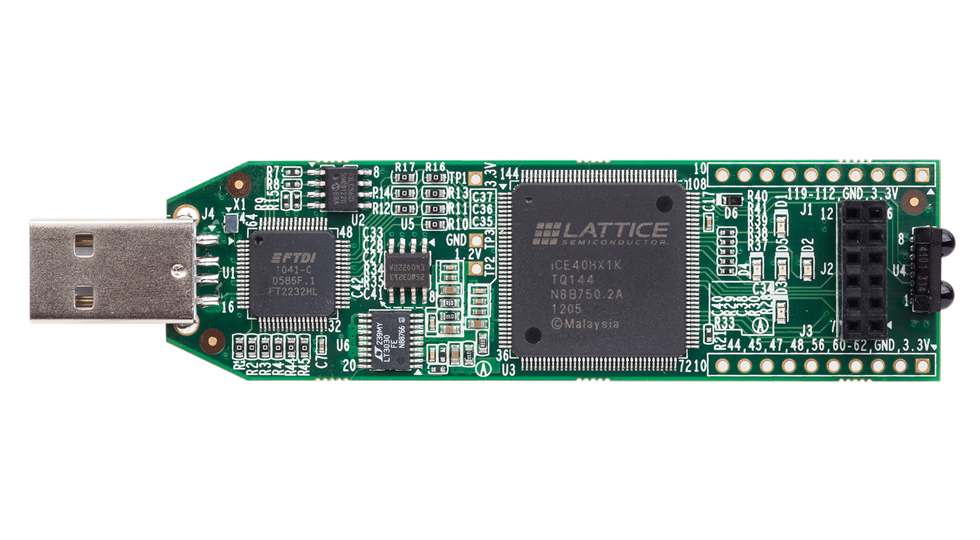
\includegraphics[width=0.8\textwidth]{icestick-reva-front-2400.png}
\end{center}

J1a SwapForth is a 16-bit version of SwapForth,
intended as an interactive Forth system using very little logic and RAM.
The system currently fits on a Lattice iCE40HX-1k FPGA. \index{FPGA}
The J1a and peripherals use 1200 logic elements.
SwapForth uses 4.7 Kbytes of RAM,
leaving about 3.3 Kbytes for the application. \index{RAM}

After installing the \index{icestorm} \index{icestorm} \index{git} \index{iceprog}
\href{http://www.clifford.at/icestorm/}{icestorm}
tools, you can run on a
\href{http://www.latticesemi.com/icestick}{Lattice iCEstick}
like this

\begin{framed}
\begin{Verbatim}
  git clone git@github.com:jamesbowman/swapforth.git
  cd swapforth/j1a
  iceprog icestorm/j1a.bin
  python shell.py -h /dev/ttyUSB0
\end{Verbatim}
\end{framed}

\noindent
(where \mach{/dev/ttyUSB0} is the appropriate port your iCEstick was assigned).
You should see something like

\begin{framed}
\begin{Verbatim}
  Contacting... established
  Loaded 208 words
  >
\end{Verbatim}
\end{framed}

And you can now try the usual Forth things, e.g.

\begin{framed}
\begin{Verbatim}[commandchars=\\\{\}]
\underline{\textbf{1 2 + .}}
3   ok
\end{Verbatim}
\end{framed}

There is a fairly complete 
\href{http://forth.sourceforge.net/std/dpans/dpans6.htm}{core ANS-compatible Forth system}
running on the board, including a compiler.

\section{Some demos} \index{demos}

You can control the five on-board LEDs \index{LEDs}

\begin{framed}
\begin{Verbatim}[commandchars=\\\{\}]
\underline{\textbf{-1 leds}}
  ok

\underline{\textbf{0 leds}}
  ok
\end{Verbatim}
\end{framed}

\noindent
and to make them blink

\begin{framed}
\begin{Verbatim}[commandchars=\\\{\}]
: blink
  32 0 do
    i leds
    100 ms
  loop
;
blink
\end{Verbatim}
\end{framed}

There is an
\href{http://www.wilbaden.com/neil_bawd/easter.txt}{Easter date calculator}
\index{easter} \index{computus@\textit{computus}}

\begin{framed}
\begin{Verbatim}
    new
    #include ../demos/easter.fs
\end{Verbatim}
\end{framed}
    
Now you can do

\begin{framed}
\begin{Verbatim}
    >2015 .easter
    2015 April 5   ok
\end{Verbatim}
\end{framed}

Or even

\begin{framed}
\begin{Verbatim}
    >: 20easters
    +  2035 2015 do
    +    cr i .easter
    +  loop
    +;
     ok
    >20easters

    2015 April 5 
    2016 March 27 
    2017 April 16 
    2018 April 1 
    2019 April 21 
    2020 April 12 
    2021 April 4 
    2022 April 17 
    2023 April 9 
    2024 March 31 
    2025 April 20 
    2026 April 5 
    2027 March 28 
    2028 April 16 
    2029 April 1 
    2030 April 21 
    2031 April 13 
    2032 March 28 
    2033 April 17 
    2034 April 9   ok
\end{Verbatim}
\end{framed}

\section{Building from Scratch}

After installing the icestorm tools, run

\begin{Verbatim}
rm build/*
make -C icestorm
\end{Verbatim}

\noindent
This will produce \mach{j1a.bin} - but it only contains the very bare-bones system;
the rest of SwapForth still needs to be compiled.
To do this, load \mach{j1a.bin} and start the shell:

\begin{framed}
\begin{Verbatim}
  $ iceprog icestorm/j1a.bin
  $ python shell.py -h /dev/ttyUSB0 -p ../common/
  Contacting... established
  Loaded 127 words
  >
\end{Verbatim}
\end{framed}

Then compile the rest of SwapForth and write the finished executable with these commands:

\begin{framed}
\begin{Verbatim}
  #include swapforth.fs
  #flash build/nuc.hex
  #bye
\end{Verbatim}
\end{framed}

Now run \mach{make -C icestorm} again - this compiles an FPGA image with the complete code base built-in.

%%%%%%%%%%%%%%%%%%%%%%%%%%%%%%%%%%%%%%%%%%%%%%%%%%%%%%%%%%%%%%%%%%%%%%%%

\newcommand{\worddef}[3]{
% \begin{samepage}
\vspace{1pt}
\noindent \word{#1} \mach{#2} #3
\\
}

\newcommand{\longworddef}[3]{
\begin{samepage}
\vspace{1pt}

\noindent \word{#1}
\index{#1@\mach{#1}}

\vspace{4pt}

\mach{#2}

\vspace{4pt}

\setlength{\parindent}{0cm}

#3

\end{samepage}

\noindent
\textcolor{lightgray}{\rule{\textwidth}{1pt}}
}

\chapter{Available Words}

\section{ANS Core Words} \index{ANS}

J1a SwapForth implements most of the core ANS 94 Forth standard.
Implemented words are:

\href{http://forth.sourceforge.net/std/dpans/dpans6.htm#6.1.0010}{\word{!}}
\href{http://forth.sourceforge.net/std/dpans/dpans6.htm#6.1.0030}{\word{\#}}
\href{http://forth.sourceforge.net/std/dpans/dpans6.htm#6.1.0040}{\word{\#>}}
\href{http://forth.sourceforge.net/std/dpans/dpans6.htm#6.1.0050}{\word{\#s}}
\href{http://forth.sourceforge.net/std/dpans/dpans6.htm#6.1.0070}{\word{'}}
\href{http://forth.sourceforge.net/std/dpans/dpans6.htm#6.1.0080}{\word{(}}
\href{http://forth.sourceforge.net/std/dpans/dpans6.htm#6.1.0090}{\word{*}}
\href{http://forth.sourceforge.net/std/dpans/dpans6.htm#6.1.0100}{\word{*/}}
\href{http://forth.sourceforge.net/std/dpans/dpans6.htm#6.1.0110}{\word{*/mod}}
\href{http://forth.sourceforge.net/std/dpans/dpans6.htm#6.1.0120}{\word{+}}
\href{http://forth.sourceforge.net/std/dpans/dpans6.htm#6.1.0130}{\word{+!}}
\href{http://forth.sourceforge.net/std/dpans/dpans6.htm#6.1.0140}{\word{+loop}}
\href{http://forth.sourceforge.net/std/dpans/dpans6.htm#6.1.0150}{\word{,}}
\href{http://forth.sourceforge.net/std/dpans/dpans6.htm#6.1.0160}{\word{-}}
\href{http://forth.sourceforge.net/std/dpans/dpans6.htm#6.1.0180}{\word{.}}
\href{http://forth.sourceforge.net/std/dpans/dpans6.htm#6.1.0190}{\word{."}}
\href{http://forth.sourceforge.net/std/dpans/dpans6.htm#6.1.0230}{\word{/}}
\href{http://forth.sourceforge.net/std/dpans/dpans6.htm#6.1.0240}{\word{/mod}}
\href{http://forth.sourceforge.net/std/dpans/dpans6.htm#6.1.0250}{\word{0<}}
\href{http://forth.sourceforge.net/std/dpans/dpans6.htm#6.1.0270}{\word{0=}}
\href{http://forth.sourceforge.net/std/dpans/dpans6.htm#6.1.0290}{\word{1+}}
\href{http://forth.sourceforge.net/std/dpans/dpans6.htm#6.1.0300}{\word{1-}}
\href{http://forth.sourceforge.net/std/dpans/dpans6.htm#6.1.0310}{\word{2!}}
\href{http://forth.sourceforge.net/std/dpans/dpans6.htm#6.1.0320}{\word{2*}}
\href{http://forth.sourceforge.net/std/dpans/dpans6.htm#6.1.0330}{\word{2/}}
\href{http://forth.sourceforge.net/std/dpans/dpans6.htm#6.1.0350}{\word{2@}}
\href{http://forth.sourceforge.net/std/dpans/dpans6.htm#6.1.0370}{\word{2drop}}
\href{http://forth.sourceforge.net/std/dpans/dpans6.htm#6.1.0380}{\word{2dup}}
\href{http://forth.sourceforge.net/std/dpans/dpans6.htm#6.1.0400}{\word{2over}}
\href{http://forth.sourceforge.net/std/dpans/dpans6.htm#6.1.0430}{\word{2swap}}
\href{http://forth.sourceforge.net/std/dpans/dpans6.htm#6.1.0450}{\word{:}}
\href{http://forth.sourceforge.net/std/dpans/dpans6.htm#6.1.0460}{\word{;}}
\href{http://forth.sourceforge.net/std/dpans/dpans6.htm#6.1.0480}{\word{<}}
\href{http://forth.sourceforge.net/std/dpans/dpans6.htm#6.1.0490}{\word{<\#}}
\href{http://forth.sourceforge.net/std/dpans/dpans6.htm#6.1.0530}{\word{=}}
\href{http://forth.sourceforge.net/std/dpans/dpans6.htm#6.1.0540}{\word{>}}
\href{http://forth.sourceforge.net/std/dpans/dpans6.htm#6.1.0550}{\word{>body}}
\href{http://forth.sourceforge.net/std/dpans/dpans6.htm#6.1.0560}{\word{>in}}
\href{http://forth.sourceforge.net/std/dpans/dpans6.htm#6.1.0570}{\word{>number}}
\href{http://forth.sourceforge.net/std/dpans/dpans6.htm#6.1.0580}{\word{>r}}
\href{http://forth.sourceforge.net/std/dpans/dpans6.htm#6.1.0630}{\word{?dup}}
\href{http://forth.sourceforge.net/std/dpans/dpans6.htm#6.1.0650}{\word{@}}
\href{http://forth.sourceforge.net/std/dpans/dpans6.htm#6.1.0670}{\word{abort}}
% \href{http://forth.sourceforge.net/std/dpans/dpans6.htm#6.1.0680}{\word{abort"}}
\href{http://forth.sourceforge.net/std/dpans/dpans6.htm#6.1.0690}{\word{abs}}
\href{http://forth.sourceforge.net/std/dpans/dpans6.htm#6.1.0695}{\word{accept}}
\href{http://forth.sourceforge.net/std/dpans/dpans6.htm#6.1.0705}{\word{align}}
\href{http://forth.sourceforge.net/std/dpans/dpans6.htm#6.1.0706}{\word{aligned}}
\href{http://forth.sourceforge.net/std/dpans/dpans6.htm#6.1.0710}{\word{allot}}
\href{http://forth.sourceforge.net/std/dpans/dpans6.htm#6.1.0720}{\word{and}}
\href{http://forth.sourceforge.net/std/dpans/dpans6.htm#6.1.0750}{\word{base}}
\href{http://forth.sourceforge.net/std/dpans/dpans6.htm#6.1.0760}{\word{begin}}
\href{http://forth.sourceforge.net/std/dpans/dpans6.htm#6.1.0770}{\word{bl}}
\href{http://forth.sourceforge.net/std/dpans/dpans6.htm#6.1.0850}{\word{c!}}
\href{http://forth.sourceforge.net/std/dpans/dpans6.htm#6.1.0860}{\word{c,}}
\href{http://forth.sourceforge.net/std/dpans/dpans6.htm#6.1.0870}{\word{c@}}
\href{http://forth.sourceforge.net/std/dpans/dpans6.htm#6.1.0880}{\word{cell+}}
\href{http://forth.sourceforge.net/std/dpans/dpans6.htm#6.1.0890}{\word{cells}}
\href{http://forth.sourceforge.net/std/dpans/dpans6.htm#6.1.0895}{\word{char}}
\href{http://forth.sourceforge.net/std/dpans/dpans6.htm#6.1.0897}{\word{char+}}
\href{http://forth.sourceforge.net/std/dpans/dpans6.htm#6.1.0898}{\word{chars}}
\href{http://forth.sourceforge.net/std/dpans/dpans6.htm#6.1.0950}{\word{constant}}
\href{http://forth.sourceforge.net/std/dpans/dpans6.htm#6.1.0980}{\word{count}}
\href{http://forth.sourceforge.net/std/dpans/dpans6.htm#6.1.0990}{\word{cr}}
\href{http://forth.sourceforge.net/std/dpans/dpans6.htm#6.1.1000}{\word{create}}
\href{http://forth.sourceforge.net/std/dpans/dpans6.htm#6.1.1170}{\word{decimal}}
\href{http://forth.sourceforge.net/std/dpans/dpans6.htm#6.1.1200}{\word{depth}}
\href{http://forth.sourceforge.net/std/dpans/dpans6.htm#6.1.1240}{\word{do}}
\href{http://forth.sourceforge.net/std/dpans/dpans6.htm#6.1.1250}{\word{does>}}
\href{http://forth.sourceforge.net/std/dpans/dpans6.htm#6.1.1260}{\word{drop}}
\href{http://forth.sourceforge.net/std/dpans/dpans6.htm#6.1.1290}{\word{dup}}
\href{http://forth.sourceforge.net/std/dpans/dpans6.htm#6.1.1310}{\word{else}}
\href{http://forth.sourceforge.net/std/dpans/dpans6.htm#6.1.1320}{\word{emit}}
% \href{http://forth.sourceforge.net/std/dpans/dpans6.htm#6.1.1345}{\word{environment?}}
\href{http://forth.sourceforge.net/std/dpans/dpans6.htm#6.1.1360}{\word{evaluate}}
\href{http://forth.sourceforge.net/std/dpans/dpans6.htm#6.1.1370}{\word{execute}}
\href{http://forth.sourceforge.net/std/dpans/dpans6.htm#6.1.1380}{\word{exit}}
\href{http://forth.sourceforge.net/std/dpans/dpans6.htm#6.1.1540}{\word{fill}}
\href{http://forth.sourceforge.net/std/dpans/dpans6.htm#6.1.1550}{\word{find}}
\href{http://forth.sourceforge.net/std/dpans/dpans6.htm#6.1.1561}{\word{fm/mod}}
\href{http://forth.sourceforge.net/std/dpans/dpans6.htm#6.1.1650}{\word{here}}
\href{http://forth.sourceforge.net/std/dpans/dpans6.htm#6.1.1670}{\word{hold}}
\href{http://forth.sourceforge.net/std/dpans/dpans6.htm#6.1.1680}{\word{i}}
\href{http://forth.sourceforge.net/std/dpans/dpans6.htm#6.1.1700}{\word{if}}
\href{http://forth.sourceforge.net/std/dpans/dpans6.htm#6.1.1710}{\word{immediate}}
\href{http://forth.sourceforge.net/std/dpans/dpans6.htm#6.1.1720}{\word{invert}}
\href{http://forth.sourceforge.net/std/dpans/dpans6.htm#6.1.1730}{\word{j}}
\href{http://forth.sourceforge.net/std/dpans/dpans6.htm#6.1.1750}{\word{key}}
\href{http://forth.sourceforge.net/std/dpans/dpans6.htm#6.1.1760}{\word{leave}}
\href{http://forth.sourceforge.net/std/dpans/dpans6.htm#6.1.1780}{\word{literal}}
\href{http://forth.sourceforge.net/std/dpans/dpans6.htm#6.1.1800}{\word{loop}}
\href{http://forth.sourceforge.net/std/dpans/dpans6.htm#6.1.1805}{\word{lshift}}
\href{http://forth.sourceforge.net/std/dpans/dpans6.htm#6.1.1810}{\word{m*}}
\href{http://forth.sourceforge.net/std/dpans/dpans6.htm#6.1.1870}{\word{max}}
\href{http://forth.sourceforge.net/std/dpans/dpans6.htm#6.1.1880}{\word{min}}
\href{http://forth.sourceforge.net/std/dpans/dpans6.htm#6.1.1890}{\word{mod}}
\href{http://forth.sourceforge.net/std/dpans/dpans6.htm#6.1.1900}{\word{move}}
\href{http://forth.sourceforge.net/std/dpans/dpans6.htm#6.1.1910}{\word{negate}}
\href{http://forth.sourceforge.net/std/dpans/dpans6.htm#6.1.1980}{\word{or}}
\href{http://forth.sourceforge.net/std/dpans/dpans6.htm#6.1.1990}{\word{over}}
\href{http://forth.sourceforge.net/std/dpans/dpans6.htm#6.1.2033}{\word{postpone}}
\href{http://forth.sourceforge.net/std/dpans/dpans6.htm#6.1.2050}{\word{quit}}
\href{http://forth.sourceforge.net/std/dpans/dpans6.htm#6.1.2060}{\word{r>}}
\href{http://forth.sourceforge.net/std/dpans/dpans6.htm#6.1.2070}{\word{r@}}
\href{http://forth.sourceforge.net/std/dpans/dpans6.htm#6.1.2120}{\word{recurse}}
\href{http://forth.sourceforge.net/std/dpans/dpans6.htm#6.1.2140}{\word{repeat}}
\href{http://forth.sourceforge.net/std/dpans/dpans6.htm#6.1.2160}{\word{rot}}
\href{http://forth.sourceforge.net/std/dpans/dpans6.htm#6.1.2162}{\word{rshift}}
\href{http://forth.sourceforge.net/std/dpans/dpans6.htm#6.1.2165}{\word{s"}}
\href{http://forth.sourceforge.net/std/dpans/dpans6.htm#6.1.2170}{\word{s>d}}
\href{http://forth.sourceforge.net/std/dpans/dpans6.htm#6.1.2210}{\word{sign}}
\href{http://forth.sourceforge.net/std/dpans/dpans6.htm#6.1.2214}{\word{sm/rem}}
\href{http://forth.sourceforge.net/std/dpans/dpans6.htm#6.1.2216}{\word{source}}
\href{http://forth.sourceforge.net/std/dpans/dpans6.htm#6.1.2220}{\word{space}}
\href{http://forth.sourceforge.net/std/dpans/dpans6.htm#6.1.2230}{\word{spaces}}
\href{http://forth.sourceforge.net/std/dpans/dpans6.htm#6.1.2250}{\word{state}}
\href{http://forth.sourceforge.net/std/dpans/dpans6.htm#6.1.2260}{\word{swap}}
\href{http://forth.sourceforge.net/std/dpans/dpans6.htm#6.1.2270}{\word{then}}
\href{http://forth.sourceforge.net/std/dpans/dpans6.htm#6.1.2310}{\word{type}}
\href{http://forth.sourceforge.net/std/dpans/dpans6.htm#6.1.2320}{\word{u.}}
\href{http://forth.sourceforge.net/std/dpans/dpans6.htm#6.1.2340}{\word{u<}}
\href{http://forth.sourceforge.net/std/dpans/dpans6.htm#6.1.2360}{\word{um*}}
\href{http://forth.sourceforge.net/std/dpans/dpans6.htm#6.1.2370}{\word{um/mod}}
\href{http://forth.sourceforge.net/std/dpans/dpans6.htm#6.1.2380}{\word{unloop}}
\href{http://forth.sourceforge.net/std/dpans/dpans6.htm#6.1.2390}{\word{until}}
\href{http://forth.sourceforge.net/std/dpans/dpans6.htm#6.1.2410}{\word{variable}}
\href{http://forth.sourceforge.net/std/dpans/dpans6.htm#6.1.2430}{\word{while}}
\href{http://forth.sourceforge.net/std/dpans/dpans6.htm#6.1.2450}{\word{word}}
\href{http://forth.sourceforge.net/std/dpans/dpans6.htm#6.1.2490}{\word{xor}}
\href{http://forth.sourceforge.net/std/dpans/dpans6.htm#6.1.2500}{\word{[}}
\href{http://forth.sourceforge.net/std/dpans/dpans6.htm#6.1.2510}{\word{[']}}
\href{http://forth.sourceforge.net/std/dpans/dpans6.htm#6.1.2520}{\word{[char]}}
\href{http://forth.sourceforge.net/std/dpans/dpans6.htm#6.1.2540}{\word{]}}

\noindent
These core words
\word{abort"}
\word{environment?}
are not implemented.
J1a SwapForth also implements the following standard words:

\href{http://forth.sourceforge.net/std/dpans/dpans6.htm#6.2.0200}{\wordidx{.(}}
\href{http://forth.sourceforge.net/std/dpans/dpans6.htm#6.2.0210}{\wordidx{.r}}
\href{http://forth.sourceforge.net/std/dpans/dpans15.htm#15.6.1.0220}{\wordidx{.s}}
\href{http://forth.sourceforge.net/std/dpans/dpans17.htm#17.6.1.0245}{\wordidx{/string}}
\href{http://forth.sourceforge.net/std/dpans/dpans6.htm#6.2.0260}{\wordidx{0<>}}
\href{http://forth.sourceforge.net/std/dpans/dpans6.htm#6.2.0280}{\wordidx{0>}}
\href{http://forth.sourceforge.net/std/dpans/dpans6.htm#6.2.0455}{\wordidx{:noname}}
\href{http://forth.sourceforge.net/std/dpans/dpans6.htm#6.2.0500}{\wordidx{<>}}
\href{http://forth.sourceforge.net/std/dpans/dpans6.htm#6.2.0620}{\wordidx{?do}}
\href{http://forth.sourceforge.net/std/dpans/dpans6.htm#6.2.0700}{\wordidx{again}}
\href{http://forth.sourceforge.net/std/dpans/dpans15.htm#15.6.2.0702}{\wordidx{ahead}}
\href{http://forth.sourceforge.net/std/dpans/dpans6.htm#6.2.0873}{\wordidx{case}}
\href{http://forth.sourceforge.net/std/dpans/dpans17.htm#17.6.1.0910}{\wordidx{cmove}}
\href{http://forth.sourceforge.net/std/dpans/dpans17.htm#17.6.1.0920}{\wordidx{cmove>}}
\href{http://forth.sourceforge.net/std/dpans/dpans6.htm#6.2.0945}{\wordidx{compile,}}
\href{http://forth.sourceforge.net/std/dpans/dpans8.htm#8.6.1.1040}{\wordidx{d+}}
\href{http://forth.sourceforge.net/std/dpans/dpans8.htm#8.6.1.1060}{\wordidx{d.}}
\href{http://forth.sourceforge.net/std/dpans/dpans8.htm#8.6.1.1070}{\wordidx{d.r}}
\href{http://forth.sourceforge.net/std/dpans/dpans8.htm#8.6.1.1080}{\wordidx{d0=}}
\href{http://forth.sourceforge.net/std/dpans/dpans8.htm#8.6.1.1090}{\wordidx{d2*}}
\href{http://forth.sourceforge.net/std/dpans/dpans8.htm#8.6.1.1160}{\wordidx{dabs}}
\href{http://forth.sourceforge.net/std/dpans/dpans8.htm#8.6.1.1230}{\wordidx{dnegate}}
\href{http://forth.sourceforge.net/std/dpans/dpans15.htm#15.6.1.1280}{\wordidx{dump}}
\href{http://forth.sourceforge.net/std/dpans/dpans6.htm#6.2.1342}{\wordidx{endcase}}
\href{http://forth.sourceforge.net/std/dpans/dpans6.htm#6.2.1343}{\wordidx{endof}}
\href{http://forth.sourceforge.net/std/dpans/dpans6.htm#6.2.1350}{\wordidx{erase}}
\href{http://forth.sourceforge.net/std/dpans/dpans6.htm#6.2.1485}{\wordidx{false}}
\href{http://forth.sourceforge.net/std/dpans/dpans6.htm#6.2.1660}{\wordidx{hex}}
\href{http://forth.sourceforge.net/std/dpans/dpans10.htm#10.6.1.1755}{\wordidx{key?}}
\href{http://forth.sourceforge.net/std/dpans/dpans8.htm#8.6.1.1830}{\wordidx{m+}}
\href{http://forth.sourceforge.net/std/dpans/dpans6.htm#6.2.1850}{\wordidx{marker}}
\href{http://forth.sourceforge.net/std/dpans/dpans10.htm#10.6.2.1905}{\wordidx{ms}}
\href{http://forth.sourceforge.net/std/dpans/dpans6.htm#6.2.1930}{\wordidx{nip}}
\href{http://forth.sourceforge.net/std/dpans/dpans6.htm#6.2.1950}{\wordidx{of}}
\href{http://forth.sourceforge.net/std/dpans/dpans6.htm#6.2.2000}{\wordidx{pad}}
\href{http://forth.sourceforge.net/std/dpans/dpans6.htm#6.2.2008}{\wordidx{parse}}
\href{http://forth.sourceforge.net/std/dpans/dpans6.htm#6.2.2125}{\wordidx{refill}}
\href{http://forth.sourceforge.net/std/dpans/dpans6.htm#6.2.2148}{\wordidx{restore-input}}
\href{http://forth.sourceforge.net/std/dpans/dpans6.htm#6.2.2182}{\wordidx{save-input}}
\href{http://forth.sourceforge.net/std/dpans/dpans17.htm#17.6.1.2212}{\wordidx{sliteral}}
\href{http://forth.sourceforge.net/std/dpans/dpans9.htm#9.6.1.2275}{\wordidx{throw}}
\href{http://forth.sourceforge.net/std/dpans/dpans6.htm#6.2.2298}{\wordidx{true}}
\href{http://forth.sourceforge.net/std/dpans/dpans6.htm#6.2.2300}{\wordidx{tuck}}
\href{http://forth.sourceforge.net/std/dpans/dpans6.htm#6.2.2330}{\wordidx{u.r}}
\href{http://forth.sourceforge.net/std/dpans/dpans6.htm#6.2.2350}{\wordidx{u>}}
\href{http://forth.sourceforge.net/std/dpans/dpans6.htm#6.2.2395}{\wordidx{unused}}
\href{http://forth.sourceforge.net/std/dpans/dpans6.htm#6.2.2440}{\wordidx{within}}
\href{http://forth.sourceforge.net/std/dpans/dpans15.htm#15.6.1.2465}{\wordidx{words}}
\href{http://forth.sourceforge.net/std/dpans/dpans6.htm#6.2.2530}{\wordidx{[compile]}}
\href{http://forth.sourceforge.net/std/dpans/dpans6.htm#6.2.2535}{\wordidx{\textbackslash}}

\noindent
Double numbers are supported using the standard \mach{.} suffix.
The Forth 200x number prefixes are supported: \index{Forth 200x}
\mach{\$} for hex,
\mach{\#} for decimal,
\mach{\%} for binary, and \mach{'c'} for character literals.
\href{http://www.forth200x.org/parse-name.html}{\wordidx{parse-name}}
is also implemented.

\newpage
\section{Additional Words}

The following words are not standard.
Some are traditional Forth words, others are specific to the J1a SwapForth implementation.

\vspace{10pt}

\longworddef{.x}{( n -- )}{display n as a 4-digit hex number}
\longworddef{-rot}{( x1 x2 x3 -- x3 x1 x2 )}{rotate the top three stack entries}
\longworddef{bounds}{( start cnt -- start+cnt start )}{prepare to loop on a range}
\longworddef{forth}{( -- a )}{variable: most recent dictionary entry}
\longworddef{io!}{( x a -- )}{store \mach{x} to IO port \mach{a}}
\longworddef{io@}{( a -- x )}{fetch from IO port \mach{a}}
\longworddef{leds}{( x -- )}{write \mach{x} to the onboard LEDs}
\longworddef{new}{( -- )}{restore code and data pointers to the power-up state}
\longworddef{s,}{( a u -- )}{add the \mach{u}-character string \mach{a} to the data space}
\longworddef{serialize}{( -- )}{display all of current memory in base 36}
% \worddef{sfind}{( dir pin -- )}{Like standard word \mach{find}, but uses a
\longworddef{tth}{( -- a )}{variable: tethered mode}

\chapter{Using SwapForth}

\section{Raw UART access}

At boot, SwapForth listens for a command on the UART. \index{UART}
Connection parameters are 115200 8N1, and any terminal program should be able to connect.
\index{DTR} \index{reset}
Note that the hardware board uses DTR as a reset signal, so you should make sure that it is set OFF by the terminal program:

\begin{verbatim}
$ miniterm.py --dtr=0 /dev/ttyUSB5 115200
--- Miniterm on /dev/ttyUSB5: 115200,8,N,1 ---
--- Quit: Ctrl+]  |  Menu: Ctrl+T | Help: Ctrl+T followed by Ctrl+H ---
--- forcing DTR inactive

  ok
  ok
  ok
\end{verbatim}

% Raw UART access does not provide the conveniences of the SwapForth shell.

\section{The SwapForth shell} \index{shell}

The SwapForth shell is a Python program that runs on the host PC.
It has a number of advantages over raw UART access:

\begin{itemize}
\item command-line editing
\item command history
\item word completion on TAB
\item local file \mach{include}
\item \mach{\^{}C} for interrupt
\end{itemize}

\subsection{Command reference}

\newcommand{\shcmd}[2]{
  \subsubsection{\mach{\##1} - #2}
  \index{#1@\mach{\##1}}
  \index{\##1@\mach{\##1}}
}
\shcmd{bye}{quit SwapForth shell}
\shcmd{flash}{copy the target state to a local file}
\shcmd{include}{send local source file}
\shcmd{noverbose}{turn off include echo}
\shcmd{time}{measure execution time}

\section{Tethered Mode}

J1a SwapForth supports
\term{tethered mode},
which makes the UART protocol easier to use for host programs.
The SwapForth shell uses
tethered mode.
To enter tethered mode, write one to the variable \wordidx{tth}:

\begin{framed}
\begin{Verbatim}
1 tth !
\end{Verbatim}
\end{framed}

In tethered mode, \word{accept} transmits byte value 30 (hex \mach{1e}, ASCII code RS).
This allows the listening program to know that the target machine is ready to accept a line of input.
In addition, \word{accept} does not echo characters as they are typed.

\chapter{Memory}

\section{Memory map}

The J1a SwapForth implementation uses 8Kbytes of RAM for code and data. \index{RAM}
The standard Forth words access this RAM.
Cells are 16-bits, and must be aligned to a 16-bit boundary.

\newpage
\section{Dictionary Layout} \index{dictionary}

\vspace{10pt}
\noindent
\begin{bytefield}[endianness=big, bitwidth=2.0em]{16}
  \bitheader{0-15} \\
    \bitbox{15}{next pointer} & \bitbox{1}{\small{imm}} \\
    \bitbox{8}{name$_1$} & \bitbox{8}{count} \\
    \bitbox{16}{...} \\
    \bitbox{8}{name$_n$} & \bitbox{8}{name$_{n-1}$} \\
    \bitbox[lr]{16}{start of word's code} \\
    \bitbox[lr]{16}{...} \\
    \bitbox[lrb]{16}{} \\
\end{bytefield}

The SwapForth dictionary is a linked list;
the variable \mach{forth} holds the start of this list.
Each dictionary entry has the following fields:

\begin{itemize}
\item \textbf{next pointer} - address of the next dictionary entry, or zero for the last dictionary entry
\item \textbf{imm} - immediate bit, set if the word is immediate
\item \textbf{count} - length of the name, in characters, 1-31
\item \textbf{name$_1$ - name$_n$} - characters in name. If the length of the name is even, then a padding byte is appended
\end{itemize}

\chapter{iCEstick Hardware interface}

\begin{center}
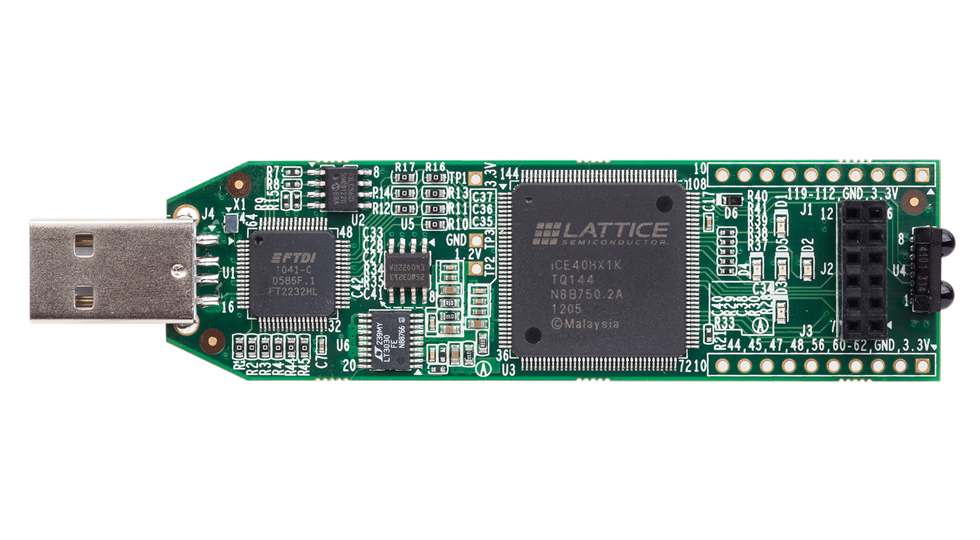
\includegraphics[width=0.8\textwidth]{icestick-reva-front-2400.png}
\end{center}

The J1a for iCEstick includes connections to the iCEstick peripherals:
\begin{itemize}
\item SPI flash \index{SPI flash}
\item LEDs \index{LEDs}
\item IrDA tranceiver \index{IrDA}
\item \digilentpmod{} connector \index{Pmod}
% \item prototyping connectors
\item UART \index{UART}
\end{itemize}

Access to peripherals is via the
\mach{io@} and \mach{io!} words.
Peripherals are port-mapped into a 16-bit IO address space.
Most ports are either read-only or write-only.
For read-only ports, writing to the port has no effect.
For write-only ports, reading from the port gives zero.

As an example of direct port access, this word
blinks the on-board LEDs when a signal on IrDA is detected. \index{blink}

\begin{framed}
\begin{Verbatim}
: x
  begin
    $2000 io@     \ read from input port
    8 and 0=      \ true if bit 3 (IrDA RXD) is 0
    $0004 io!     \ write to LEDS
  again
;
\end{Verbatim}
\end{framed}

\newpage
\section{Port Map}
\subsection{\$0001: \digilentpmod{} data}

The read-write port at address \$0001 is for direct access to the \digilentpmod{}
connector. The port pins are assigned:

\vspace{10pt}
\begin{tabular}{cccc}
\textbf{connection} & \textbf{Left row pins} & \textbf{right row pins} & \textbf{connection} \\
\hline
bit 0 & 1 &  7 & bit 4 \\
bit 1 & 2 &  8 & bit 5 \\
bit 2 & 3 &  9 & bit 6 \\
bit 3 & 4 & 10 & bit 7 \\
ground & 5 & 11 & ground \\
3.3v & 6 & 12 & 3.3v \\
\end{tabular}
\vspace{10pt}

Correspondingly the port bits are assigned to pins as follows:

\vspace{10pt}
\noindent
\begin{bytefield}[endianness=big, bitwidth=2.0em]{16}
  \bitheader{0-15} \\
    \bitbox{8}{} &
    \bitbox{1}{10} &
    \bitbox{1}{9} &
    \bitbox{1}{8} &
    \bitbox{1}{7} &
    \bitbox{1}{4} &
    \bitbox{1}{3} &
    \bitbox{1}{2} &
    \bitbox{1}{1}
\end{bytefield}
\vspace{10pt}

Note that pin direction is controlled by the corresponding bit the port at address \$0002.

\subsection{\$0002: \digilentpmod{} direction}

Each of the 8 bits controls the direction of the corresponding pin of the \digilentpmod{} connector.
0 sets the pin to input, 1 means sets the pin to output.
The bit-to-pin mapping is the same as for port \$0001.

\subsection{\$0004: LEDs}

The five on-board LEDS are controlled by write-only port at address \$0004.
Setting a bit to 1 lights the corresponding LED.

\vspace{10pt}
\noindent
\begin{bytefield}[endianness=big, bitwidth=2.0em]{16}
  \bitheader{0-15} \\
    \bitbox{11}{} &
    \bitbox{1}{\tiny{LED5}} &
    \bitbox{1}{\tiny{LED4}} &
    \bitbox{1}{\tiny{LED3}} &
    \bitbox{1}{\tiny{LED2}} &
    \bitbox{1}{\tiny{LED1}}
\end{bytefield}

Built-in word
\wordidx{leds}
writes to this port.

\subsection{\$0008: PIO output}

%  assign {PIO1_20, PIO1_18, PIOS_00, PIOS_02, PIOS_03} = PIOS;

Write-only port \$0008 controls the flash and IrDA outputs.

\vspace{10pt}
\noindent
\begin{bytefield}[endianness=big, bitwidth=2.0em]{16}
  \bitheader{0-15} \\
    \bitbox{11}{} &
    \bitbox{1}{\tiny{IrDA\\SD}} &
    \bitbox{1}{\tiny{IrDA\\TXD}} &
    \bitbox{1}{\tiny{flash\\SCK}} &
    \bitbox{1}{\tiny{flash\\MOSI}} &
    \bitbox{1}{\tiny{flash\\CS}}
\end{bytefield}


\subsection{\$1000: UART data}

The read-write port at address \$1000 is for UART transmission or reception.
Writing to the port starts transmission of a byte, reading the port returns
the incoming byte.

Standard words
\wordidx{key}, \wordidx{key?} and \wordidx{emit}
can be used to access this port.

\vspace{10pt}
\noindent
\begin{bytefield}[endianness=big, bitwidth=2.0em]{16}
  \bitheader{0-15} \\
    \bitbox{8}{} &
    \bitbox{8}{byte}
\end{bytefield}

\subsection{\$2000: IrDA, flash and UART inputs}

Read-only port \$2000 contains the input signals from the
IrDA receiver, SPI flash, and UART.

\vspace{10pt}
\noindent
\begin{bytefield}[endianness=big, bitwidth=2.0em]{16}
  \bitheader{0-15} \\
    \bitbox{12}{} &
    \bitbox{1}{\tiny{IrDA\\RXD}} &
    \bitbox{1}{\tiny{flash\\MISO}} &
    \bitbox{1}{\tiny{UART\\key?}} &
    \bitbox{1}{\tiny{UART\\busy}}
\end{bytefield}

\clearpage
\addcontentsline{toc}{chapter}{Index}
\printindex

\end{document}
